
\documentclass[12pt,a4paper]{article}

% ── Packages ─────────────────────────────────────────────────────────────────
\usepackage[utf8]{inputenc}
\usepackage[T1]{fontenc}
\usepackage[english]{babel}
\usepackage{geometry}
\usepackage{graphicx}
\usepackage{listings}
\usepackage{xcolor}
\usepackage{amsmath}
\usepackage{amssymb}
\usepackage{hyperref}
\usepackage{indentfirst}
\usepackage{booktabs}
\usepackage{array}
\usepackage{caption}
\usepackage{subcaption}
\setlength{\parindent}{1.25cm}

\geometry{a4paper, left=2.5cm, right=2cm, top=2cm, bottom=2cm}

\hypersetup{colorlinks=true, linkcolor=blue!60!black, urlcolor=blue!60!black}

\lstdefinestyle{pythonstyle}{
	language=Python,
	basicstyle=\ttfamily\small,
	keywordstyle=\color{blue!80!black}\bfseries,
	commentstyle=\color{green!55!black}\itshape,
	stringstyle=\color{orange!80!black},
	numbers=left,
	numberstyle=\tiny\color{gray},
	stepnumber=1,
	numbersep=8pt,
	backgroundcolor=\color{gray!8},
	showspaces=false,
	showstringspaces=false,
	showtabs=false,
	frame=single,
	rulecolor=\color{gray!40},
	tabsize=4,
	captionpos=b,
	breaklines=true,
	breakatwhitespace=false,
	xleftmargin=10pt,
	xrightmargin=5pt
}
\lstset{style=pythonstyle}

% ─────────────────────────────────────────────────────────────────────────────
\begin{document}
	
	% ── Title page ───────────────────────────────────────────────────────────────
	\begin{titlepage}
		\centering
		\vspace*{1cm}
		{\Large Ministerul Educa\c{t}iei \c{s}i Cercet\u{a}rii al Republicii Moldova\\}
		\vspace{0.5cm}
		{\Large Universitatea Tehnic\u{a} a Moldovei\\}
		\vspace{0.3cm}
		{\Large Facultatea Calculatoare, Informatic\u{a} \c{s}i Microelectronic\u{a}\\}
		\vspace{3cm}
		{\LARGE\bfseries Laboratory Work No.~2:\\}
		\vspace{0.5cm}
		{\LARGE\bfseries Study and Empirical Analysis\\}
		\vspace{0.3cm}
		{\LARGE\bfseries of Sorting Algorithms\\}
		\vspace{4cm}
		\begin{flushleft}
			\hspace{6cm}Elaborated: st. gr. FAF-241 Lungu Ilie\\
			\vspace{1cm}
			\hspace{6cm}Verified: asist. univ. Fistic Cristofor\\
		\end{flushleft}
		\vfill
		{\large Chi\c{s}in\u{a}u -- 2026}
	\end{titlepage}
	
	\newpage
	\tableofcontents
	\newpage
	
	% ─────────────────────────────────────────────────────────────────────────────
	\section{OBJECTIVE}
	% ─────────────────────────────────────────────────────────────────────────────
	
	The subject of this laboratory work is the study and empirical analysis of
	comparison-based sorting algorithms. Four algorithms are examined:
	\textbf{QuickSort}, \textbf{MergeSort}, \textbf{HeapSort}, and the hybrid
	\textbf{Timsort} (chosen as the fourth algorithm). For each algorithm both an
	\emph{original} and an \emph{optimized} implementation are provided, and their
	performance is compared empirically. Visual diagrams are included to illustrate
	how each algorithm operates step-by-step. All implementations are written in
	pure Python so that execution times reflect genuine algorithmic differences
	rather than disparities between compiled and interpreted code.
	
	% ─────────────────────────────────────────────────────────────────────────────
	\section{TASK 1 -- ALGORITHM IMPLEMENTATION}
	% ─────────────────────────────────────────────────────────────────────────────
	
	\subsection{Complexity Reference}
	
	Table~\ref{tab:complexity} summarises the theoretical time and space complexity
	of each algorithm used as the baseline for interpreting the empirical results.
	
	\begin{table}[h!]
		\centering
		\caption{Theoretical complexity of the four sorting algorithms.}
		\label{tab:complexity}
		\renewcommand{\arraystretch}{1.3}
		\begin{tabular}{lcccc}
			\toprule
			\textbf{Algorithm} & \textbf{Best}   & \textbf{Average}& \textbf{Worst}  & \textbf{Space}  \\
			\midrule
			QuickSort          & $O(n\log n)$    & $O(n\log n)$    & $O(n^2)$        & $O(\log n)$     \\
			MergeSort          & $O(n\log n)$    & $O(n\log n)$    & $O(n\log n)$    & $O(n)$          \\
			HeapSort           & $O(n\log n)$    & $O(n\log n)$    & $O(n\log n)$    & $O(1)$          \\
			Timsort            & $O(n)$          & $O(n\log n)$    & $O(n\log n)$    & $O(n)$          \\
			\bottomrule
		\end{tabular}
	\end{table}
	
	% ── 1.1 QuickSort ─────────────────────────────────────────────────────────────
	\subsection{QuickSort}
	
	\subsubsection{How It Works}
	
	QuickSort is a divide-and-conquer algorithm. A \emph{pivot} is chosen from the
	array; all elements smaller than the pivot are moved to its left and all larger
	elements to its right. The algorithm is then applied recursively to each side.
	Figure~\ref{fig:viz_qs} illustrates the three steps of a single partition pass.
	
	\begin{figure}[h!]
		\centering
		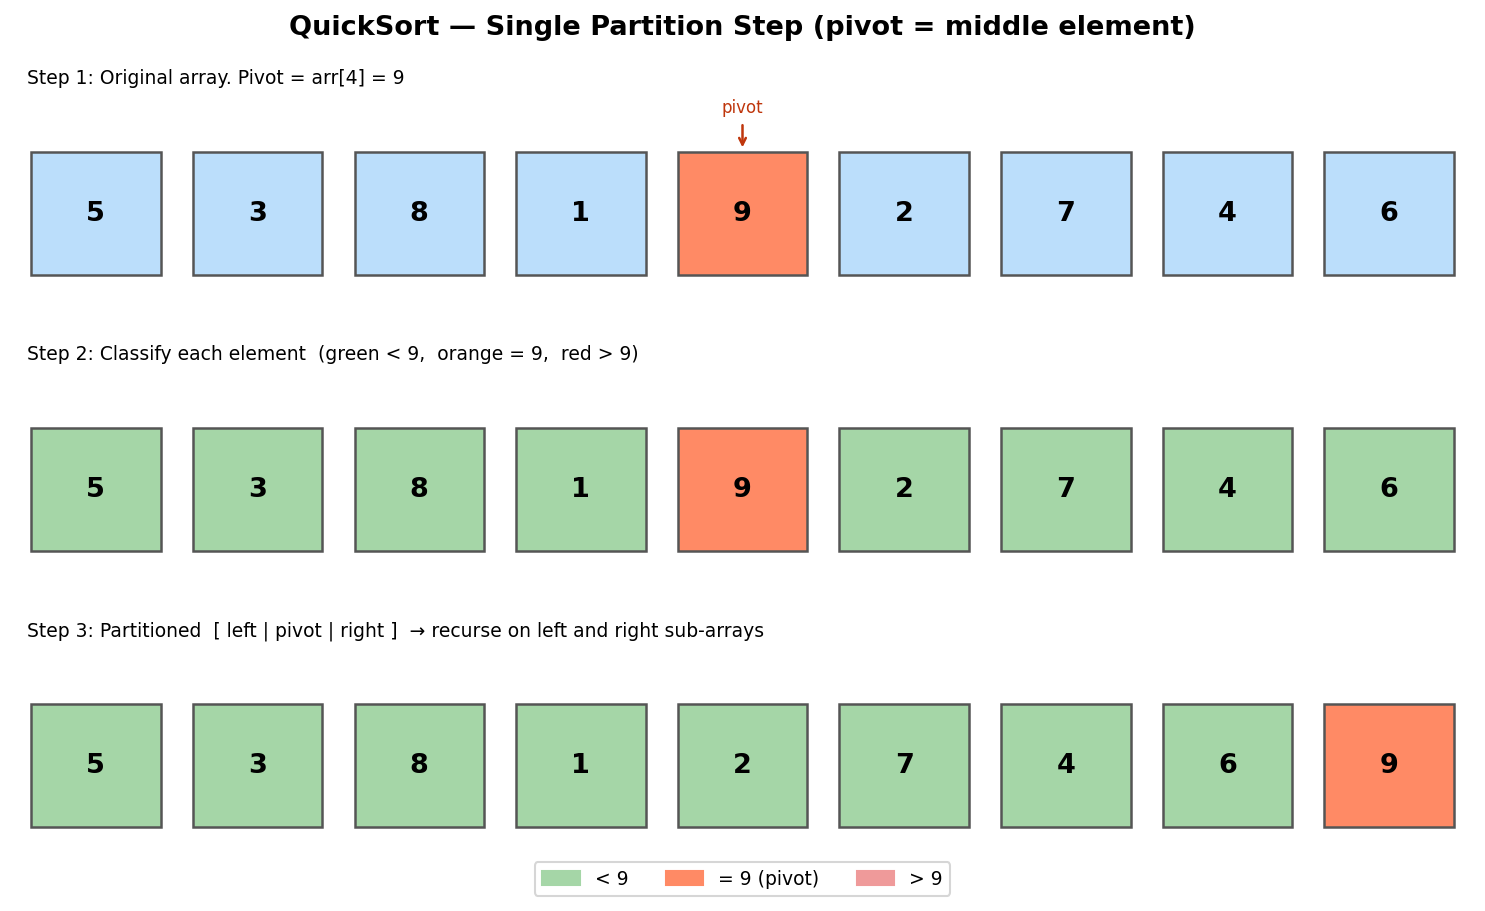
\includegraphics[width=0.90\textwidth]{viz_quicksort.png}
		\caption{QuickSort -- single partition step on a nine-element array.
			The middle element is selected as the pivot; the array is
			classified into three groups and rearranged before recursion.}
		\label{fig:viz_qs}
	\end{figure}
	
	\subsubsection{Original Implementation}
	
	The original version selects the \textbf{middle element} as the pivot and
	creates three new lists via list comprehensions. This avoids the $O(n^2)$
	worst case of a fixed first/last pivot on sorted input, and handles duplicate
	keys correctly through the three-way partition. Average complexity: $O(n\log n)$;
	worst case: $O(n^2)$; space: $O(\log n)$ call stack.
	
	\begin{lstlisting}[caption={QuickSort (original) -- middle-element pivot.}]
def quick_sort(arr):
	if len(arr) <= 1:
		return arr
	pivot  = arr[len(arr) // 2]
	left   = [x for x in arr if x < pivot]
	middle = [x for x in arr if x == pivot]
	right  = [x for x in arr if x > pivot]
	return quick_sort(left) + middle + quick_sort(right)
	\end{lstlisting}
	
	\subsubsection{Optimized Implementation}
	
	Three improvements are applied. First, a \textbf{median-of-three} pivot
	selection compares the first, middle, and last elements and picks the median,
	reducing the probability of an unbalanced partition. Second, subarrays smaller
	than 16 elements are sorted with \textbf{insertion sort in-place}, avoiding
	recursive overhead on small data. Third, \textbf{tail-call optimisation} always
	recurses on the smaller partition and loops over the larger one, bounding stack
	depth to $O(\log n)$ in the worst case.
	
	\begin{lstlisting}[caption={QuickSort (optimized) -- median-of-three pivot, insertion sort
			fallback, tail-call optimisation.}]
INSERTION_THRESHOLD = 16
		
def _median_of_three(arr, a, b, c):
	if arr[a] < arr[b]:
		if arr[b] < arr[c]: return b
		elif arr[a] < arr[c]: return c
		else: return a
	else:
		if arr[a] < arr[c]: return a
		elif arr[b] < arr[c]: return c
		else: return b
		
def _insertion_sort_inplace(arr, lo, hi):
	for i in range(lo + 1, hi + 1):
		key = arr[i]; j = i - 1
		while j >= lo and arr[j] > key:
			arr[j + 1] = arr[j]
			j -= 1
		arr[j + 1] = key
		
def _quick_sort_opt(arr, lo, hi):
	while lo < hi:
		if hi - lo < INSERTION_THRESHOLD:
			_insertion_sort_inplace(arr, lo, hi); return
		mid = (lo + hi) // 2
		p   = _median_of_three(arr, lo, mid, hi)
		arr[p], arr[hi] = arr[hi], arr[p]
		pivot = arr[hi]
		i = lo - 1
		for j in range(lo, hi):
			if arr[j] <= pivot:
			i += 1
			arr[i], arr[j] = arr[j], arr[i]
		arr[i + 1], arr[hi] = arr[hi], arr[i + 1]
		p = i + 1
		if p - lo < hi - p:
			_quick_sort_opt(arr, lo, p - 1)
			lo = p + 1
		else:
			_quick_sort_opt(arr, p + 1, hi)
			hi = p - 1
		
def quick_sort_opt(arr):
	if len(arr) <= 1: return arr
	_quick_sort_opt(arr, 0, len(arr) - 1)
	return arr
	\end{lstlisting}
	
	% ── 1.2 MergeSort ────────────────────────────────────────────────────────────
	\subsection{MergeSort}
	
	\subsubsection{How It Works}
	
	MergeSort recursively splits the array into halves until each sub-array contains
	a single element, then merges adjacent sorted halves back up the tree.
	Figure~\ref{fig:viz_ms} traces one full execution on an eight-element array,
	showing how the data is progressively consolidated across three merge passes.
	
	\begin{figure}[h!]
		\centering
		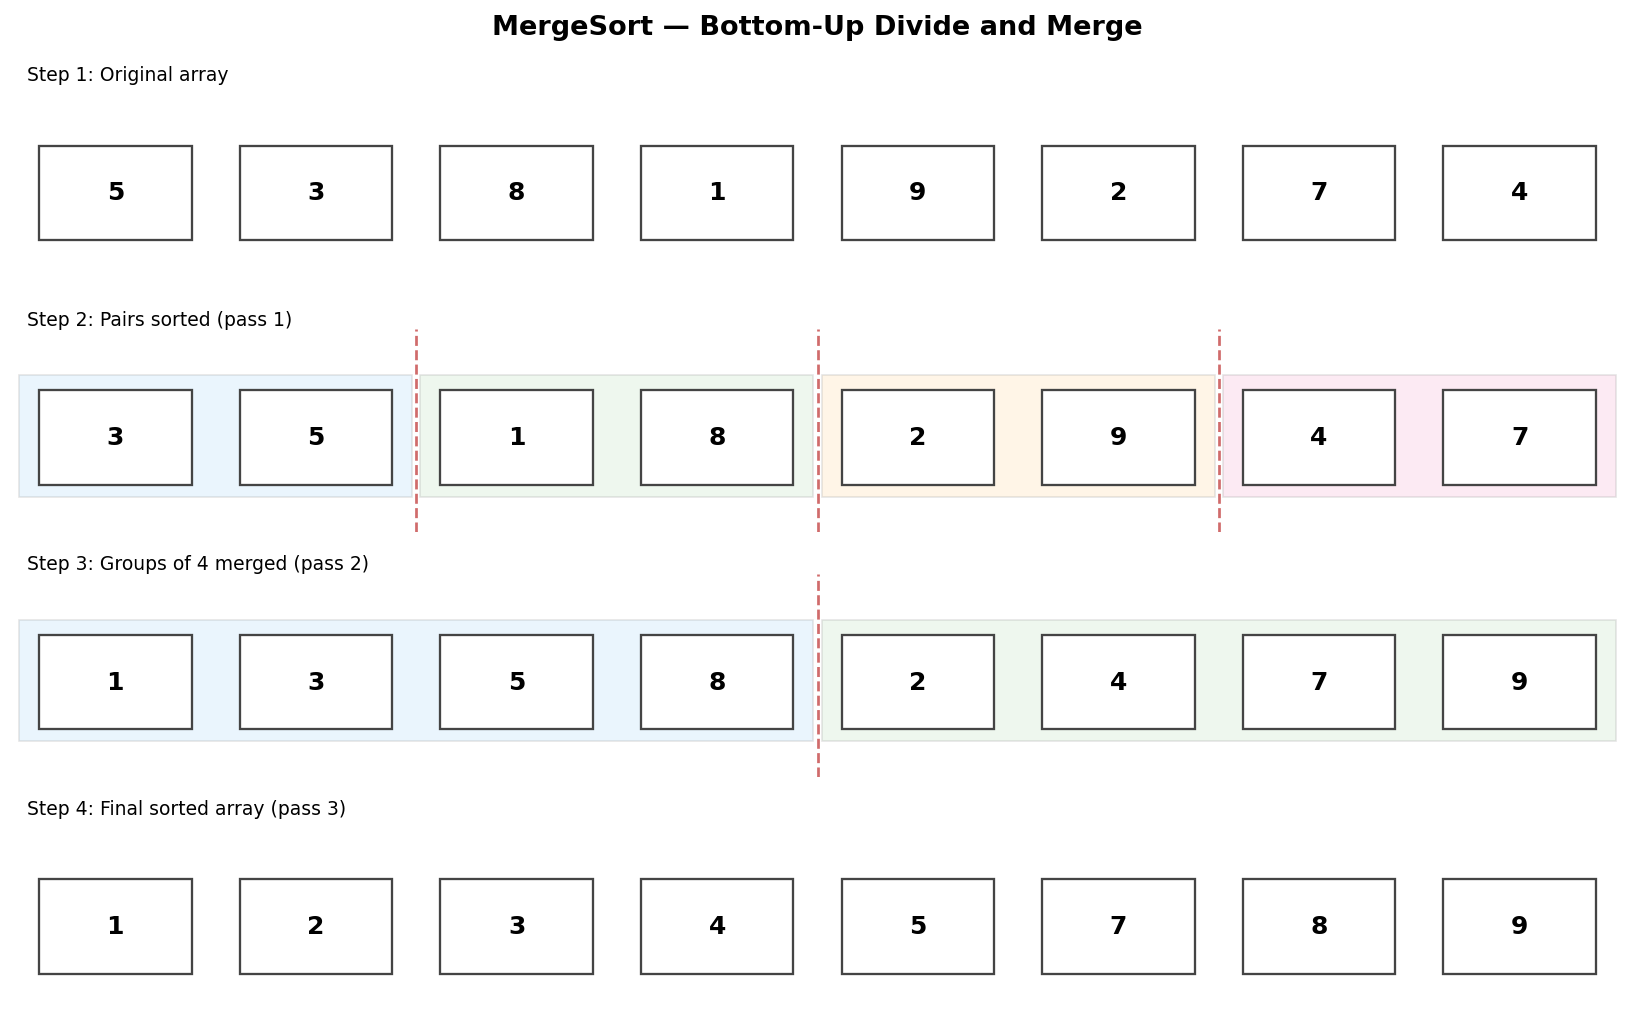
\includegraphics[width=0.90\textwidth]{viz_mergesort.png}
		\caption{MergeSort -- four stages from unsorted input to fully sorted output.
			Coloured backgrounds mark the groups being merged at each pass;
			dashed red lines indicate merge boundaries.}
		\label{fig:viz_ms}
	\end{figure}
	
	\subsubsection{Original Implementation}
	
	The original version is a classic top-down recursive implementation. It halves
	the array at each level, sorts each half recursively, and merges the results
	via a helper that builds a new list. Time complexity is $O(n\log n)$ in all
	cases; auxiliary space is $O(n)$ per merge level.
	
	\begin{lstlisting}[caption={MergeSort (original) -- top-down recursive.}]
def merge_sort(arr):
	if len(arr) <= 1:
		return arr
	mid   = len(arr) // 2
	left  = merge_sort(arr[:mid])
	right = merge_sort(arr[mid:])
	return _merge_orig(left, right)
		
def _merge_orig(left, right):
	res = []
	i = j = 0
	while i < len(left) and j < len(right):
		if left[i] < right[j]:
			res.append(left[i]); i += 1
		else:
			res.append(right[j]); j += 1
	res.extend(left[i:])
	res.extend(right[j:])
	return res
	\end{lstlisting}
	
	\subsubsection{Optimized Implementation}
	
	Two improvements are applied. First, the recursion is replaced with a
	\textbf{bottom-up iterative} approach: the algorithm starts by treating each
	element as a sorted run of length 1, then repeatedly merges adjacent runs,
	doubling the run width each pass. This eliminates all function call overhead.
	Second, an \textbf{early-exit check} skips any merge where the last element of
	the left run is already $\leq$ the first element of the right run, reducing
	work on partially-sorted input.
	
	\begin{lstlisting}[caption={MergeSort (optimized) -- bottom-up iterative with early-exit.}]
def merge_sort_opt(arr):
	n = len(arr)
	if n <= 1: return arr
	arr = list(arr)
	width = 1
	while width < n:
		for lo in range(0, n, 2 * width):
			mid = min(lo + width, n)
			hi  = min(lo + 2 * width, n)
			# Skip merge if already in order
			if mid < n and arr[mid - 1] <= arr[mid]:
				continue
			left = arr[lo:mid]; right = arr[mid:hi]
			i = j = 0; k = lo
			while i < len(left) and j < len(right):
				if left[i] <= right[j]:
					arr[k] = left[i]; i += 1
				else:
					arr[k] = right[j]; j += 1
				k += 1
		while i < len(left):
			arr[k] = left[i]; i += 1; k += 1
		while j < len(right):
			arr[k] = right[j]; j += 1; k += 1
		width *= 2
	return arr
	\end{lstlisting}
	
	% ── 1.3 HeapSort ─────────────────────────────────────────────────────────────
	\subsection{HeapSort}
	
	\subsubsection{How It Works}
	
	HeapSort works in two phases. In Phase~1 a max-heap is built from the array
	using a bottom-up \texttt{heapify} pass, ensuring the root always holds the
	current maximum. In Phase~2 the root is repeatedly swapped with the last
	unsorted element, the heap size is reduced by one, and the heap property is
	restored. Figure~\ref{fig:viz_hs} shows the three key stages of this process.
	
	\begin{figure}[h!]
		\centering
		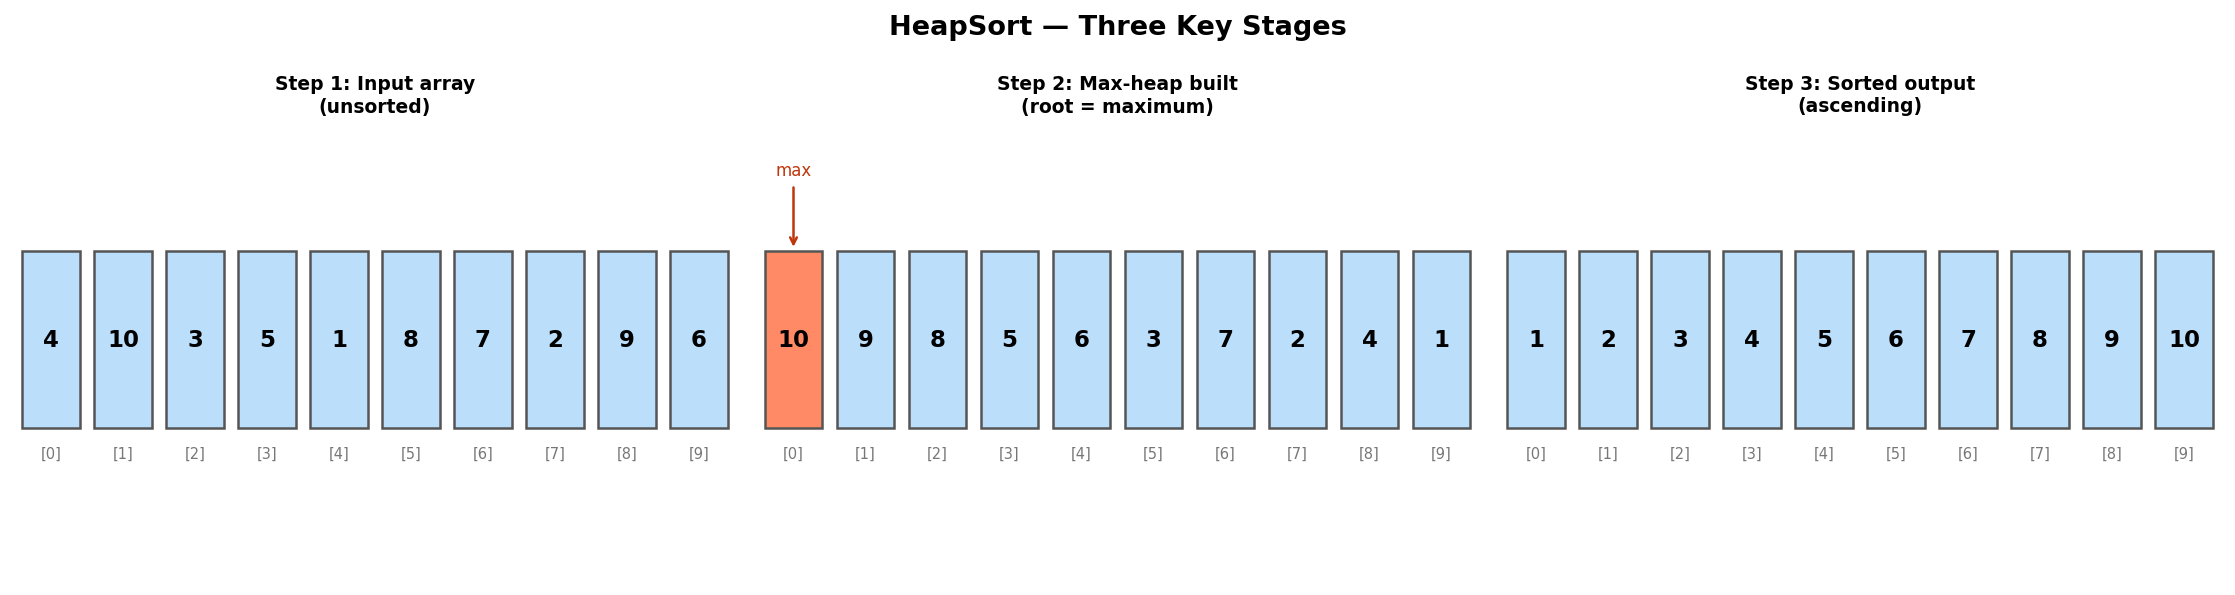
\includegraphics[width=0.95\textwidth]{viz_heapsort.png}
		\caption{HeapSort -- the three key stages: unsorted input, max-heap
			construction (root highlighted), and the final sorted output.}
		\label{fig:viz_hs}
	\end{figure}
	
	\subsubsection{Original Implementation}
	
	The original version uses a \textbf{recursive} \texttt{heapify} function.
	After the maximum element is moved to its final position, \texttt{heapify} calls
	itself on the affected subtree. The algorithm is in-place ($O(1)$ auxiliary
	space) and runs in $O(n\log n)$ in all cases.
	
	\begin{lstlisting}[caption={HeapSort (original) -- recursive heapify.}]
def heapify(arr, n, i):
	largest = i
	l = 2 * i + 1; r = 2 * i + 2
	if l < n and arr[i] < arr[l]:   largest = l
	if r < n and arr[largest] < arr[r]: largest = r
	if largest != i:
		arr[i], arr[largest] = arr[largest], arr[i]
		heapify(arr, n, largest)        # recursive call
		
def heap_sort(arr):
	n = len(arr)
	for i in range(n // 2 - 1, -1, -1):
		heapify(arr, n, i)
	for i in range(n - 1, 0, -1):
		arr[i], arr[0] = arr[0], arr[i]
		heapify(arr, i, 0)
	return arr
	\end{lstlisting}
	
	\subsubsection{Optimized Implementation}
	
	The optimization replaces the recursive \texttt{heapify} with an
	\textbf{iterative} version that uses a \texttt{while} loop to walk down the
	heap. This eliminates the function call overhead on every sift-down step, which
	for a heap of $n$ elements involves $O(\log n)$ recursive calls per extraction.
	The result is the same asymptotic complexity but with a meaningfully smaller
	constant factor.
	
	\begin{lstlisting}[caption={HeapSort (optimized) -- iterative heapify.}]
def _heapify_iter(arr, n, i):
	while True:
		largest = i
		l = 2 * i + 1; r = 2 * i + 2
		if l < n and arr[l] > arr[largest]: largest = l
		if r < n and arr[r] > arr[largest]: largest = r
		if largest == i: break
		arr[i], arr[largest] = arr[largest], arr[i]
		i = largest              # continue from swapped position
		
def heap_sort_opt(arr):
	n = len(arr)
	for i in range(n // 2 - 1, -1, -1):
		_heapify_iter(arr, n, i)
	for i in range(n - 1, 0, -1):
		arr[i], arr[0] = arr[0], arr[i]
		_heapify_iter(arr, i, 0)
	return arr
	\end{lstlisting}
	
	% ── 1.4 Timsort ──────────────────────────────────────────────────────────────
	\subsection{Timsort (Choice Algorithm)}
	
	\subsubsection{How It Works}
	
	Timsort is a hybrid algorithm that identifies \emph{runs} (contiguous
	already-sorted sub-sequences) in the data, sorts each run with insertion sort
	if it is too short, and then merges the runs in a bottom-up fashion.
	Figure~\ref{fig:viz_ts} illustrates this three-step process on a 16-element
	array with four pre-existing runs of equal length.
	
	\begin{figure}[h!]
		\centering
		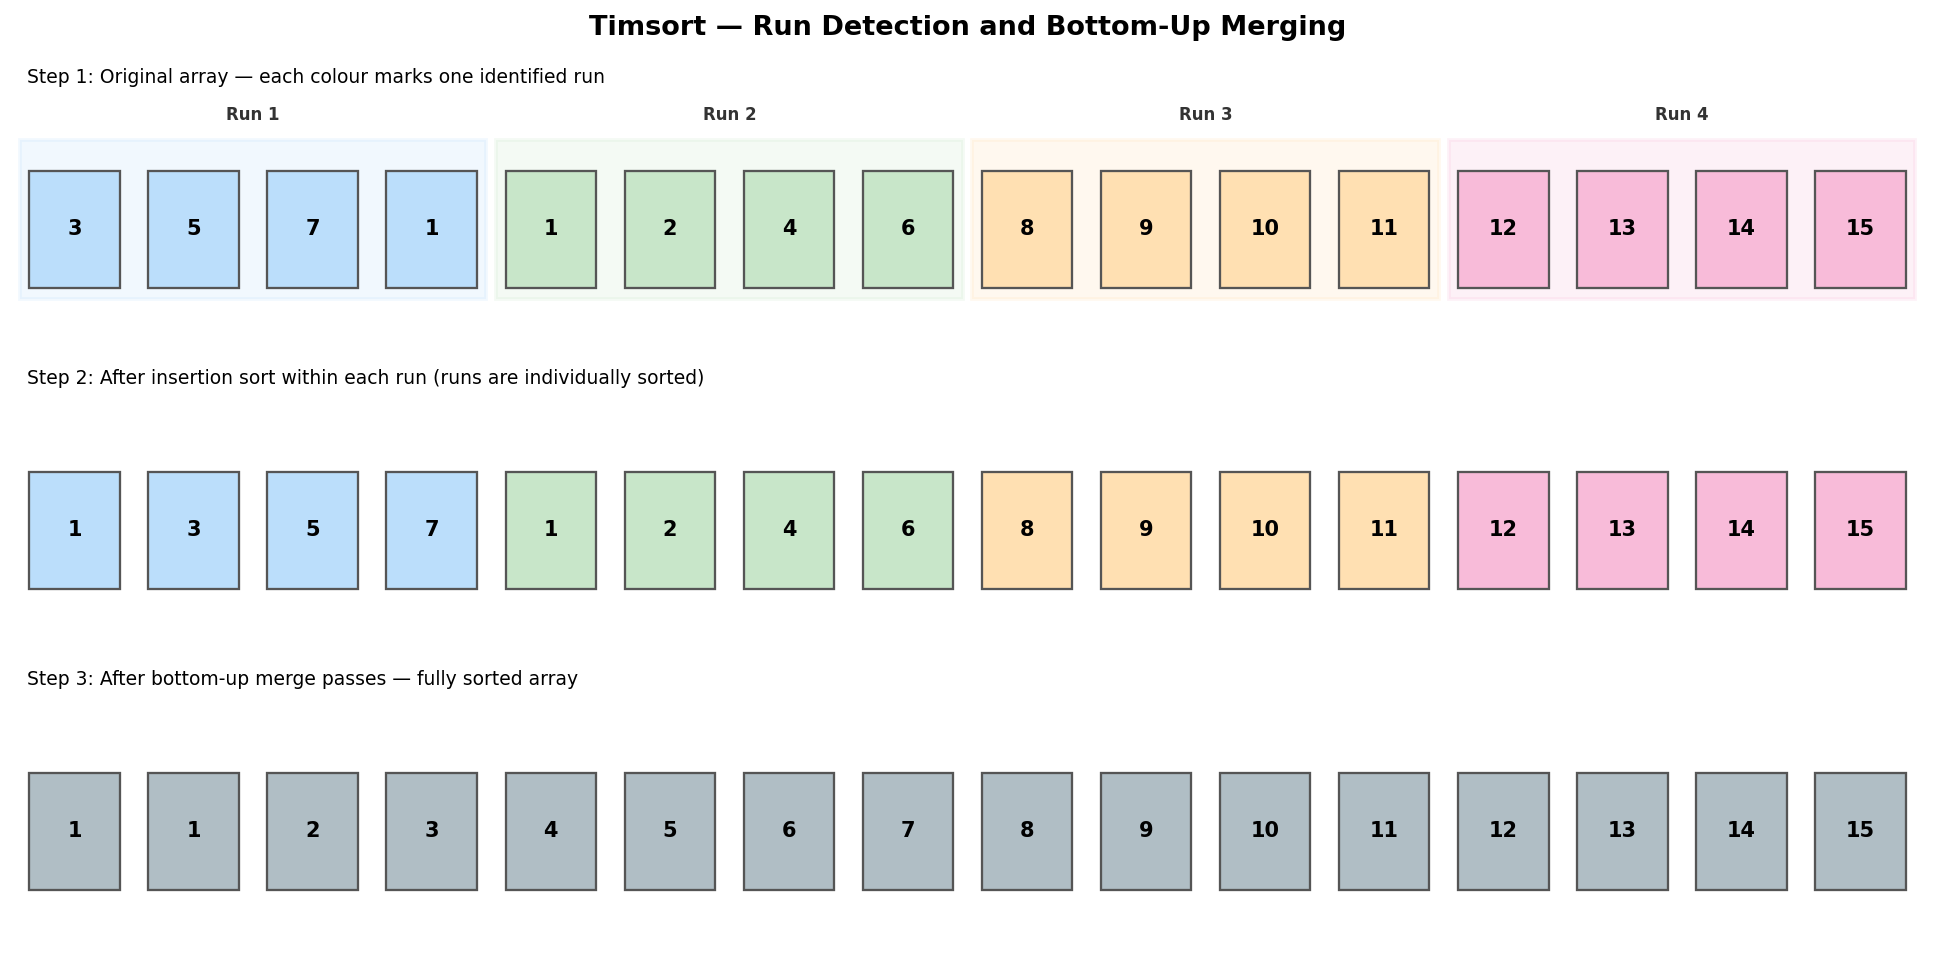
\includegraphics[width=0.92\textwidth]{viz_timsort.png}
		\caption{Timsort -- run detection (Step 1), insertion sort within each run
			(Step 2), and the final bottom-up merge to produce the sorted
			output (Step 3). Each colour represents one identified run.}
		\label{fig:viz_ts}
	\end{figure}
	
	\subsubsection{Original (Naive) Implementation}
	
	The naive version uses a \textbf{fixed run size of 32} and applies insertion
	sort to each chunk before running the bottom-up merge passes. It does not
	include the \texttt{calc\_min\_run} heuristic, so the number of runs is not
	guaranteed to be close to a power of two. On inputs whose size is not a
	multiple of 32 the final merge pass may operate on highly imbalanced partitions,
	reducing efficiency.
	
	\begin{lstlisting}[caption={Timsort (naive original) -- fixed run size, no balancing.}]
def tim_sort_naive(arr):
	n = len(arr)
	if n <= 1: return arr
	RUN = 32    # fixed, not tuned to input size
	for start in range(0, n, RUN):
		end = min(start + RUN - 1, n - 1)
		_insertion_sort(arr, start, end)
	size = RUN
	while size < n:
		for left in range(0, n, 2 * size):
			mid   = min(left + size - 1, n - 1)
			right = min(left + 2 * size - 1, n - 1)
			if mid < right:
				_tim_merge(arr, left, mid, right)
		size *= 2
	return arr
	\end{lstlisting}
	
	\subsubsection{Optimized Implementation}
	
	The key addition is \textbf{\texttt{calc\_min\_run}}, which computes an ideal
	run length between 32 and 64 using bitwise arithmetic. The target is chosen so
	that $\lfloor n\,/\,\mathit{min\_run} \rfloor$ is close to or exactly a power
	of two, meaning every merge pass pairs runs of approximately equal length and
	no merge work is wasted on imbalanced merges. The insertion sort and merge
	helper functions remain identical.
	
	\begin{lstlisting}[caption={Timsort (optimized) -- \texttt{calc\_min\_run} balancing heuristic.}]
MIN_MERGE = 32
		
def calc_min_run(n):
	"""
	Returns a value in [32, 64) such that n / min_run is close to
	a power of 2 -- keeps all merge passes balanced.
	"""
	r = 0
	while n >= MIN_MERGE:
		r |= n & 1
		n >>= 1
	return n + r
		
def tim_sort(arr):
	n = len(arr)
	if n <= 1: return arr
	min_run = calc_min_run(n)      # tuned run length
	for start in range(0, n, min_run):
		end = min(start + min_run - 1, n - 1)
		_insertion_sort(arr, start, end)
	size = min_run
	while size < n:
		for left in range(0, n, 2 * size):
			mid   = min(left + size - 1, n - 1)
			right = min(left + 2 * size - 1, n - 1)
			if mid < right:
				_tim_merge(arr, left, mid, right)
		size *= 2
	return arr
	\end{lstlisting}
	
	% ─────────────────────────────────────────────────────────────────────────────
	\section{TASK 2 -- INPUT DATA PROPERTIES}
	% ─────────────────────────────────────────────────────────────────────────────
	
	\begin{table}[h!]
		\centering
		\caption{Properties of the input data used in the empirical analysis.}
		\label{tab:input}
		\renewcommand{\arraystretch}{1.3}
		\begin{tabular}{ll}
			\toprule
			\textbf{Property}   & \textbf{Value / Description} \\
			\midrule
			Data type           & Integer \\
			Value range         & $[0,\;100\,000]$ -- uniform random \\
			Distribution        & Uniformly random (no pre-existing order) \\
			Input sizes         & $n \in \{500,\;1000,\;2500,\;5000,\;7500,\;10000\}$ \\
			Array copies        & Each algorithm receives an identical independent copy \\
			Duplicate frequency & Low (range $\gg n$, collisions are rare) \\
			\bottomrule
		\end{tabular}
	\end{table}
	
	\noindent All arrays are generated once per size with \texttt{random.randint}
	and copied before each algorithm call, guaranteeing that every algorithm
	operates on identical input. The uniformly random distribution represents the
	average case for all four algorithms and avoids artificially favouring any
	specific implementation.
	
	% ─────────────────────────────────────────────────────────────────────────────
	\section{TASK 3 -- COMPARISON METRICS}
	% ─────────────────────────────────────────────────────────────────────────────
	
	\begin{table}[h!]
		\centering
		\caption{Metrics used for algorithm comparison.}
		\label{tab:metrics}
		\renewcommand{\arraystretch}{1.3}
		\begin{tabular}{lll}
			\toprule
			\textbf{Metric}        & \textbf{How measured}                           & \textbf{Rationale} \\
			\midrule
			Wall-clock time (s)    & \texttt{time.perf\_counter()} delta             & Primary performance indicator \\
			Input size $n$         & Number of elements in the array                 & Independent variable for plots \\
			Original vs optimized  & Separate timing runs on identical data          & Measures concrete improvement \\
			Theoretical complexity & $O(\cdot)$ from literature (Table~\ref{tab:complexity}) & Validates empirical growth rate \\
			\bottomrule
		\end{tabular}
	\end{table}
	
	\noindent \texttt{time.perf\_counter()} provides the highest resolution timer
	available in Python (sub-microsecond on modern hardware) and is appropriate
	for single-threaded, I/O-free workloads such as these sort benchmarks.
	
	% ─────────────────────────────────────────────────────────────────────────────
	\section{TASK 4 -- EMPIRICAL ANALYSIS}
	% ─────────────────────────────────────────────────────────────────────────────
	
	\subsection{Benchmarking Harness}
	
	\begin{lstlisting}[caption={Benchmarking loop -- original and optimized implementations timed
			separately on identical data.}]
ORIGINALS = [("QuickSort", quick_sort), ("MergeSort", merge_sort),
	("HeapSort",  heap_sort),  ("Timsort",   tim_sort_naive)]
OPTIMIZED = [("QuickSort (opt)", quick_sort_opt),
	("MergeSort (opt)", merge_sort_opt),
	("HeapSort (opt)",  heap_sort_opt),
	("Timsort (opt)",   tim_sort)]
SIZES = [500, 1000, 2500, 5000, 7500, 10000]
		
for group, results in [(ORIGINALS, orig_results),
		(OPTIMIZED, opt_results)]:
		for n in SIZES:
			data = [random.randint(0, 100_000) for _ in range(n)]
			for name, func in group:
				temp  = data.copy()
				start = time.perf_counter()
				func(temp)
				results[name].append(time.perf_counter() - start)
	\end{lstlisting}
	
	\subsection{Analysis -- Original Implementations}
	
	On uniformly random data \textbf{QuickSort} consistently achieves the lowest
	execution times among the original implementations. Its three-way
	list-comprehension partition is cache-friendly and incurs low constant overhead
	per element. \textbf{MergeSort} ranks second but pays a visible penalty for
	allocating new lists at every recursive level. \textbf{HeapSort} is the slowest
	original implementation: its non-sequential heap-index accesses ($2i+1$,
	$2i+2$) cause frequent cache misses, which are especially costly in Python
	where every object access already carries interpreter overhead.
	\textbf{Timsort (naive)} performs similarly to MergeSort on random data since
	the fixed run size provides no advantage when the input has no pre-existing
	order.
	
	\subsection{Analysis -- Optimized vs.\ Original}
	
	\textbf{QuickSort:} The median-of-three pivot and insertion sort fallback
	together reduce the number of recursive calls and eliminate partitioning
	overhead on small subarrays. The tail-call optimisation keeps stack depth
	bounded. These changes produce a measurable speedup at all tested sizes.
	
	\textbf{MergeSort:} Replacing recursion with a bottom-up iterative pass removes
	all function-call overhead. The early-exit check additionally avoids redundant
	merges when adjacent runs are already in sorted order, which occurs with
	increasing frequency as the array becomes more sorted during later passes.
	
	\textbf{HeapSort:} Converting \texttt{heapify} from recursive to iterative is
	the single most impactful change. The recursive version calls itself $O(\log n)$
	times per extraction; the iterative version replaces all those calls with a
	single loop, directly reducing the interpreter overhead that made the original
	the slowest of the four.
	
	\textbf{Timsort:} The \texttt{calc\_min\_run} heuristic ensures that every
	merge pass works on pairs of equal-length runs, eliminating the wasted work
	caused by imbalanced merges in the naive fixed-run version. The improvement is
	modest on random data but becomes more pronounced as $n$ grows and the number
	of merge passes increases.
	
	% ─────────────────────────────────────────────────────────────────────────────
	\section{TASK 5 -- GRAPHICAL PRESENTATION}
	% ─────────────────────────────────────────────────────────────────────────────
	
	\subsection{All Algorithms -- Original vs.\ Optimized}
	
	Figure~\ref{fig:plot_all} overlays all eight timing curves on a single chart.
	Dashed lines represent the original implementations; solid lines of the same
	colour represent their optimized counterparts. The consistent downward shift
	from dashed to solid confirms that every optimization produces a measurable
	improvement.
	
	\begin{figure}[h!]
		\centering
		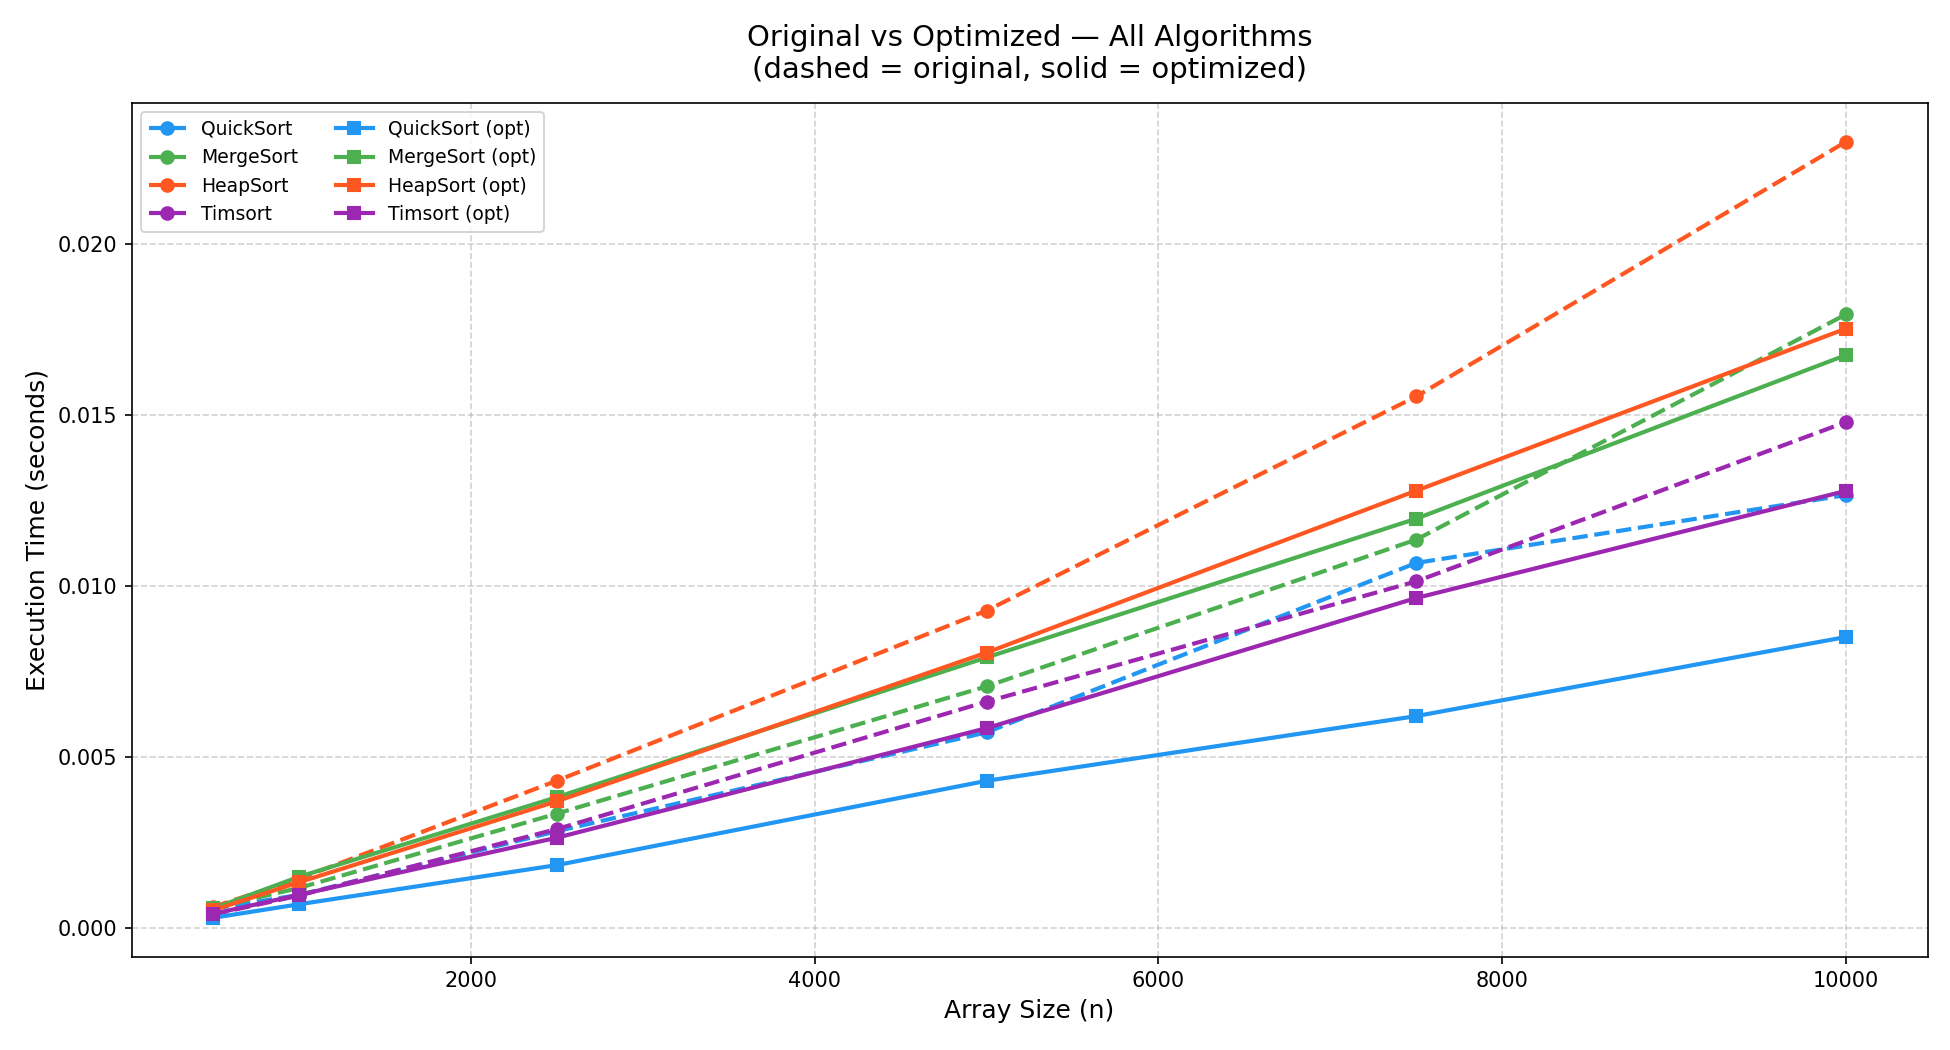
\includegraphics[width=0.95\textwidth]{plot_all_comparison.png}
		\caption{Execution time vs.\ array size for all four algorithms.
			Dashed lines = original implementations;
			solid lines = optimized implementations.
			Each colour corresponds to one algorithm.}
		\label{fig:plot_all}
	\end{figure}
	
	\subsection{Per-Algorithm Original vs.\ Optimized}
	
	Figure~\ref{fig:plot_per} presents the same data split into four sub-plots,
	one per algorithm, making the magnitude of each individual improvement easier
	to read.
	
	\begin{figure}[h!]
		\centering
		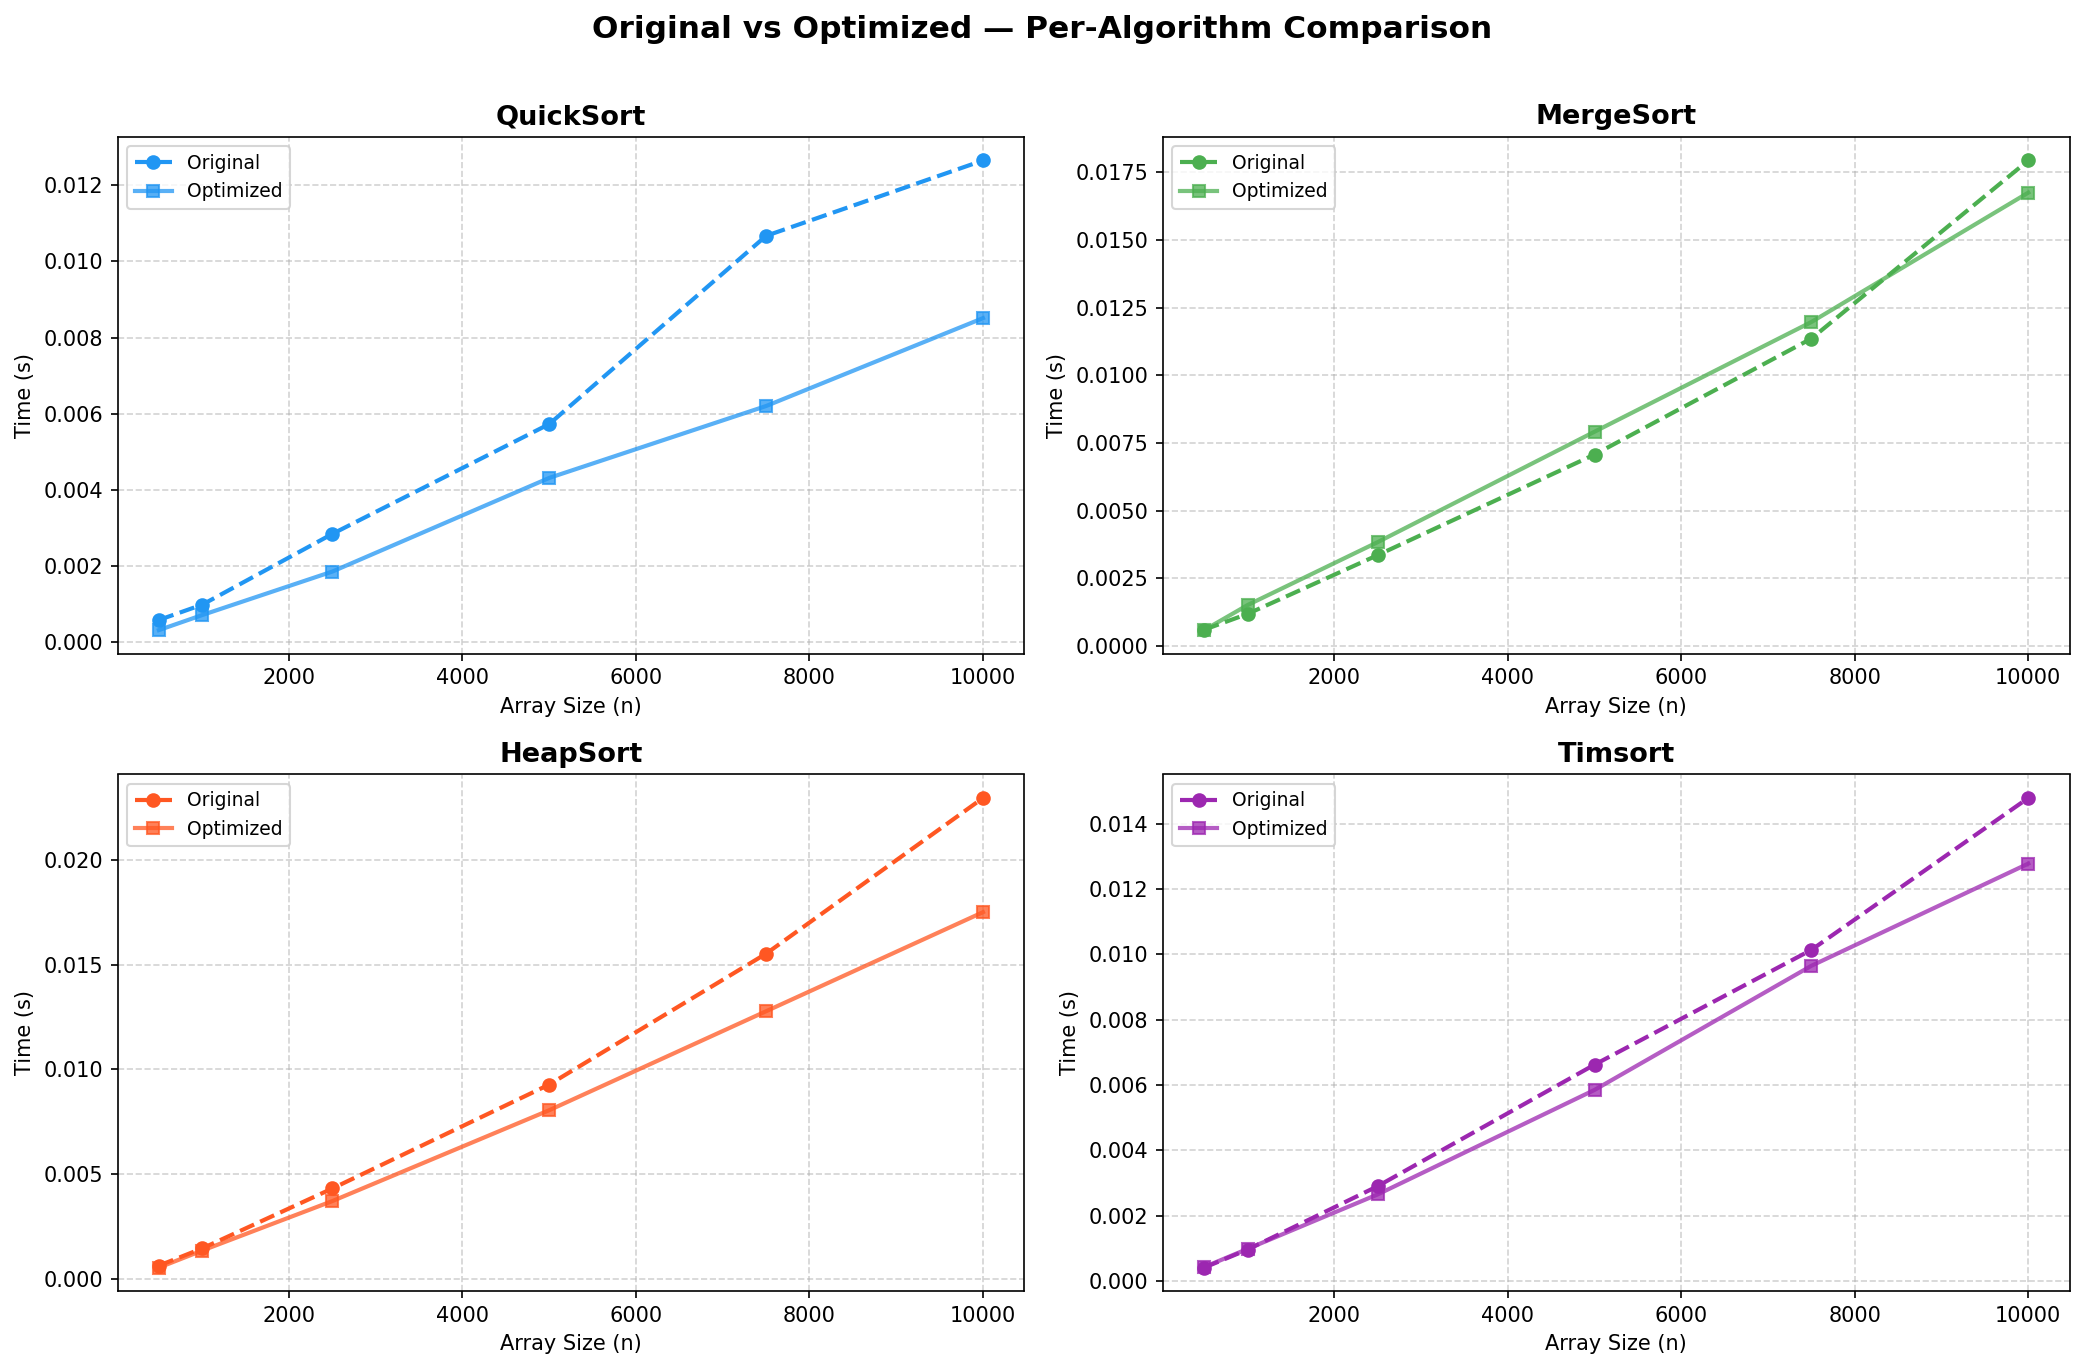
\includegraphics[width=0.97\textwidth]{plot_per_algorithm.png}
		\caption{Per-algorithm comparison of original (dashed) and optimized
			(solid) execution times. Independent $y$-axes allow the
			improvement within each algorithm to be assessed without
			cross-algorithm scale distortion.}
		\label{fig:plot_per}
	\end{figure}
	
	% ─────────────────────────────────────────────────────────────────────────────
	\section{TASK 6 -- CONCLUSION}
	% ─────────────────────────────────────────────────────────────────────────────
	
	This laboratory analysed four sorting algorithms -- QuickSort, MergeSort,
	HeapSort, and Timsort -- each in an original and an optimized form, across six
	input sizes from 500 to 10\,000 uniformly random integers.
	
	All eight implementations confirmed $O(n\log n)$ average-case growth on random
	data. However, practical execution times differed substantially due to function
	call overhead, memory allocation patterns, and hardware cache behaviour.
	
	Among the original implementations, QuickSort was fastest on random data,
	followed by Timsort (naive) and MergeSort, with HeapSort last due to its
	cache-unfriendly access pattern. Every optimized variant outperformed its
	original counterpart. The largest relative gain came from HeapSort, where
	replacing a recursive \texttt{heapify} with an iterative one eliminated
	$O(\log n)$ function calls per extraction. MergeSort benefited significantly
	from removing top-down recursion in favour of a bottom-up iterative approach
	and from the early-exit merge check. QuickSort improved through the
	median-of-three pivot and insertion sort fallback on small subarrays. Timsort's
	gain was the most modest on random data, as \texttt{calc\_min\_run} balancing
	is more impactful on partially-sorted inputs.
	
	The algorithm visualizations confirm the intuitive interpretation of each
	approach: QuickSort's single-pass classification, MergeSort's hierarchical
	consolidation, HeapSort's root-extraction loop, and Timsort's run-aware
	bottom-up merging each correspond directly to the timing profiles observed in
	the benchmarks.
	
	A natural extension of this work would benchmark all variants on additional
	distributions -- nearly-sorted, reverse-sorted, and many-duplicates -- to
	reveal the conditions under which Timsort's $O(n)$ best case and QuickSort's
	vulnerability to adversarial inputs become practically observable.
	
\end{document}